As previously mentioned, the field of gesture recognition gave birth to several image processing devices yielding useful data. One of them being Microsoft Kinect, a device where the main intention was to interpret whole-body movement, making it lacking in required accuracy for hand gesture recognition. 

\section{Leap Motion Controller}
%=======================================================================================================================
Another option would be using a Leap Motion Controller (LMC), developed specifically to track hand movements and extract its features, such as positions of fingers, hand rotation, and others.

LMC consits of two monochromatic IR cameras and three IR LEDs (emmitters). 

\begin{figure}[h]
	\centering
    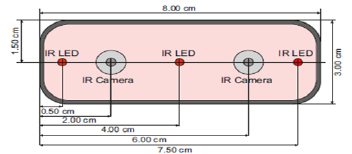
\includegraphics[width=8cm]{lmc_schematic.png}
	\caption{Schematic View of Leap Motion Controller}
	\label{fig:lmcScheme}
\end{figure}



The LMC's current API, Leap Motion Service, yields positions of extracted hand features. All the positional data about the hand and its features are represented in coordinate system relative to the LMC's center point, positioned at the middle IR LED.\cite{LMCanalysis} The x- and z-axes lie in the plane of the camera sensors, with the x-axis running along the camera baseline. The y-axis is vertical, with positive values increasing upwards (in contrast to the downward orientation of most computer graphics coordinate systems). The z-axis has positive values increasing toward the user.\cite{tomasMultileap}

\begin{figure}[h]
	\centering
    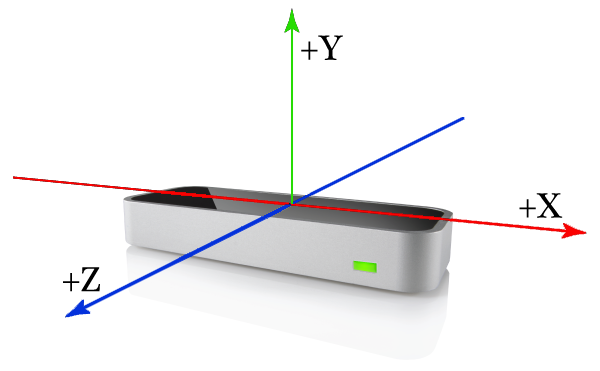
\includegraphics[width=8cm]{leap_axes.png}
	\caption{Leap Motion Controller Axes}
	\label{fig:lmcScheme}
\end{figure}


Unfortunately, Leap Motion Controller has no official library for gesture recognition, limiting developers from utilizing the controller for its key features. Orion, Leap Motion tracking software build for virtual reality, used to have a gesture detector with its 3.0 version, but the detector is absent with the release of more accurate version 4.0.